\documentclass[a4paper, 12pt]{report}

\usepackage[cache=false]{minted}
\usepackage{amsmath}
\usepackage{booktabs}
\usepackage{color}
\usepackage{enumitem}
\usepackage{examplep}
\usepackage{fancyhdr}
\usepackage{fancyvrb}
\usepackage[includeheadfoot,margin=2.5cm]{geometry}
\usepackage{multirow}
\usepackage{parskip}
\usepackage{titlesec}
\usepackage[nottoc]{tocbibind}
\usepackage{url}
\usepackage{xcolor}
\usepackage{graphicx}
\usepackage{subcaption}

\usemintedstyle{colorful}

% Choose your bibliography style
\bibliographystyle{plain}
\linespread{1.3}
% Setup headers and footers # TODO : add headers
\fancyhf{}
\fancyfoot[C] {\thepage}

\begin{document}

\graphicspath{{../doc-imgs/}}

% Front Page
\thispagestyle{empty}
\begin{center}
	\Large{
		\hfill \begin{tabular}{l}
			Computer Science\\and Mathematics\\COC255\\B827126
		\end{tabular} % #TODO: formatting for this
	}
	\vspace*{\fill}

	\Large{\textbf{TIMETABLE CREATION\\USING\\ARTIFICIAL INTELLIGENCE}}

	\vspace*{\fill}

	by

	\vspace*{\fill}

	Aiden Nico Tempest

	\vspace*{\fill}

	Supervisor: Dr.\ S. Fatima

	\vspace*{\fill}

	\underline{Department of Computer Science} \\ \underline{Loughborough
	University}

	\vspace*{\fill}
	
	August 2023

\end{center} % Front Page ends

\newpage
\begin{abstract} % #TODO: abstract
	lol placeholder text for abstract lorem ipsum etc test
\end{abstract}

% #TODO: acknowledgements

\tableofcontents

\newpage

\chapter{Introduction} % #TODO: introduction

\chapter{Literature Review}

\section{The Timetabling Problem}

The timetabling problem is a constraint satisfying problem and it is known to
be NP-Complete.
The aim is to create a university timetable where several constraints are met.
These constraints are either hard constraints or soft constraints.
For a solution to be valid, all the hard constraints must be met.
Not all (or in fact, any) of the soft constraints need to be met for the
solution to be valid, however it is preferable for as many soft constraints to
be met as possible.
Examples of possible hard constraints include:

\begin{itemize}
	\item At most only one session (i.e., a lecture or lab) is happening in a 
		specific room in a specific period
	\item A student can only be attending at most one session in a specific 
		period
	\item A teacher (e.g., a lecturer or lab helper) can only be attending at 
		most one session in a specific period
	\item The size of a student group cannot exceed the capacity of the room
	\item The room must be appropriate for the type of session, e.g., a lecture 
		must be in a lecture theatre, and a lab session must be in a computer 
		lab
	\item Part time teachers can only be assigned certain time slots, e.g., they
		may not work on Tuesdays, so sessions they teach cannot be scheduled
		for time slots on Tuesday.
\end{itemize}

Possible soft constraints include:

\begin{itemize}
	\item Students do not have more than two consecutive hours scheduled
	\item The capacity of a room is well suited to the size of the student
		group, to make an efficient use of space e.g., a group of twenty
		students are not going to be in a room with a capacity of two hundred
	\item If a student or teacher has one session immediately after another,
		then the respective rooms are relatively close to each other
\end{itemize}

A solution is invalid if at least of one the hard constraints are met.
For example, if a student is scheduled to be in two different sessions at the
same time --- this is known as a clash.

\section{Methods}

\subsection{Genetic Algorithms}

Genetic algorithms (GAs) make up a group of search metaheuristics, inspired by
Darwin's theory of evolution~\cite{ga_book}.
Here, the fittest members of a population survive and produce offspring, which
inherit the characteristics of the parents.
It is also possible for the offspring to have small mutations within their
genetic code, which may or may not be beneficial towards the population's
survival.
This theory can be applied to search problems.
In this case, the population represents the search space, which is a collection 
of candidate solutions to a problem, and the population of solutions evolves as
the algorithm searches for a desired solution.

There does not exist a rigorous definition of GAs, but most methods use these
five phases:

\begin{enumerate}
	\item Initial population --- populations of chromosomes
	\item Fitness function
	\item Selection --- according to fitness
	\item Crossover --- to produce new offspring
	\item Mutation --- random mutation of new offspring
\end{enumerate}

The initial \textbf{population} is a set of \textbf{individuals}, where each
individual represents a candidate solution to the problem.
These solutions will almost definitely not satisfy the problem, as they are
randomly generated, but that is not an issue.

An individual (and hence that candidate solution), is defined by its
\textbf{chromosome}.
The chromosome is often encoded as a string of binary characters; however, any
alphabet can be used.
These characters are called \textbf{alleles}, and a single character or group of
adjacent characters that encode a particular element of the candidate solution
are known as a \textbf{gene}.

Using the example of the university timetabling problem, several alleles may be
used to encode a room, but together they are one gene.

The \textbf{fitness} function measures how well a candidate solution solves the
problem.
For example, in the instance of the university timetabling problem, the fitness 
of the solution could be measured by the number of times in the solution that a
hard constraint is not met.
This means that a solution with a score of 0 is a valid solution, as there are
instances of a hard constraint not being met.

Once the fitness function has been used to calculate the fitness of each
individual, the fittest individuals are chosen for reproduction in the
\textbf{selection} phase.
There are several ways to select individuals to use for producing offspring.
One way is to simply choose the two individuals with the best fitness.
Another way is to use roulette-wheel sampling, where any individual could be
chosen for producing offspring, but fitter individuals are more likely to be
chosen.
This second method introduces more variation into the offspring, to reduce the
chance of convergence onto a local maximum.

The \textbf{crossover} phase, or reproduction phase, is where genetic material
is exchanged between two parents.
The crossover operator randomly chooses a locus (position) in a chromosome,
in between alleles.
The subsequent before and after parts of the chromosome are swapped between the
two parents to produce two offspring.
This is repeated multiple times to produce a population of the same size as the
initial population.
Whether this is by two parents reproducing multiple times using different loci
or not, depends on the method used in the selection phase.

After reproduction, \textbf{mutations} can be introduced into the offspring. 
For example, if the chromosomes are encoded by binary strings, then some bits 
are randomly flipped.
However, there is a very small chance of this occurring at each bit, a suggested
probability is 0.1\%.
By introducing mutations into the offspring, the likelihood of reaching a local
maximum is reduced.

Once there is a new population made up of the offspring, the process repeats 
until a solution is found.
Each repetition is called a \textbf{generation}, and the entire set of
generations is known as a \textbf{run}.

A version of a genetic algorithm was implemented by Perzina 
(2006)~\cite{ga_example} and was applied to a timetabling problem with real 
world data.
Timetables were generated for 1807 students, but for how courses are organised 
at this university, there are no groups of students with the same timetable, and
it is unlikely that two students would even have the same timetable.
Because of this, the author anticipated that it would be too difficult to
generate timetables without any clashes at all, and instead aimed to minimise
the number of clashes.
The best solution found had 83 students with at least one clash on their
timetable, or 4.59\% of the students.

\subsection{Binary Integer Programming}

Binary integer programming is used to solve constraint satisfiability problems.
Variables must either take a value of 1 or 0 (hence binary integer), as they 
are used to represent decisions, i.e., in the case of the university 
timetabling problem, a teaching session is happening in a specific room, at a 
specific time, on a specific day, with a specific teacher, with a specific 
teacher, with a specific student group, about a specific module, or 
not~\cite{bip_example}.
Then constraints are applied and used with the objective function to find what
value each variable takes.

First, a mathematical model of the problem must be constructed.
Abdellahi and Eledum (2006)~\cite{bip_example} modelled the features of the
university timetabling problem as a group of sets:
\begin{itemize}
	\item
		\begin{math}
			I = \{ 1, \dots , n_i \}
		\end{math}: set of days in the week where courses are offered
	\item
		\begin{math}
			J = \{ 1, \dots , n_j \}
		\end{math}: set of time slots in a day
	\item 
		\begin{math}
			K = \{ 1, \dots , n_k \}
		\end{math}: set of courses
	\item 
		\begin{math}
			L = \{ 1, \dots , n_l \}
		\end{math}: set of student groups
	\item 
		\begin{math}
			M = \{ 1, \dots , n_m \}
		\end{math}: set of teachers
	\item 
		\begin{math}
			N = \{ 1, \dots , n_n \}
		\end{math}: set of classrooms
\end{itemize}

Next, the decision variables are defined. The basic variables
\begin{math}
	x_{i,j,k,l,m,n}
\end{math}
are defined as
\begin{math}
	\forall i \in I, \forall j \in J, \forall k \in K, \forall l \in L, \forall
	m \in M, \forall n \in N
\end{math}
\begin{align*}
	x_{i,j,k,l,m,n} = 
	\begin{cases}
		1, & \parbox[t]{9.5cm}{if a course \( k \) taught by teacher \( m \) for
		the group of students \( l \) is assigned to the \( j^{th} \) time slot 
		of day \( i \) in classroom \( m \)} \\
		0, & \text{otherwise}
	\end{cases}
\end{align*}

In other words, the basic variables represent the decision of whether or a not
a course is being taught by a specific teacher for a specific group of students
is happening in a specific time slot of a specific day in a specific classroom.
Then the authors defined their auxiliary variables as

\begin{math}
	\forall i \in I, \forall j \in J, \forall l \in L
\end{math}
\begin{align*}
	y_{i,j,k,l} = 
	\begin{cases}
		1, & \parbox[t]{9.5cm}{if a course \( k + s \) for group of students
		overlap with its prerequite \( k \) for the same group \( l \) in the 
		\( j^{th} \) time slot of day \( i \)} \\
		0, & \text{otherwise}
	\end{cases}	
\end{align*}
\begin{math}
	\text{for } s \in 1, \ldots, n_k - 1, \text{where } k + s \leq n_k	
\end{math}

Finally, (people) defined two further sets of variables:
\begin{itemize}
	\item \( z_{im} \), which represents the existence of lectures for teacher 
		\( m \) on day \( i \)
	\item \( z_{il} \), which represents the existence of lectures for student 
		\( l \) on day \( i \)
\end{itemize}
\begin{math}
	\forall m \in M
\end{math}
\begin{align*}
	z_{im} =
	\begin{cases}
		1, & \text{if \( \sum_{j \in J} x_{i,j,k,l,m,n} \neq 0 \)} \\
		0, & \text{otherwise}
	\end{cases}	
\end{align*}
\begin{math}
	\forall l \in L
\end{math}
\begin{align*}
	z_{il} =
	\begin{cases}
		1, & \text{if \( \sum_{j \in J} x_{i,j,k,l,m,n} \neq 0 \)} \\
		0, & \text{otherwise}
	\end{cases}	
\end{align*}

\( z_{im} \) and \( z_{il} \) are for use with the object function, later. The
next thing to be modelled is the restraints.
For the university modelled by the authors, these were:

\begin{enumerate}
	\item There is no overlapping for courses
	\item Each teacher cannot be assigned to more than one course for any given
		period
	\item Each classroom cannot hold more than one course for any given period
	\item A student has some courses amount to 18 hours per week. Each course
		consists of 3 hours and taught in 2 periods (each period is 90 minutes
		long), which is expressed as the number of slots worked per day.
	\item For a student, each course occupies only one slot per day
	\item The lectures of each course must be distributed in such a way that
		there is one day off between them
	\item All lectures of a given course in a week must be held in the same
		classroom
	\item The overlap of course with prerequisites for the same group of
		undergrad students l is permitted (note: the authors refer to undergrad 
		students as pre-graduated students)
\end{enumerate}

As an example, the first restraint is modelled as:
\begin{align*}
	\sum_{k \in K} \sum_{m \in M} \sum_{n \in N} x_{i,j,k,l,m,n} \leq 1 \quad
	\forall i \in I, \forall j \in J, \forall l \in L
\end{align*}
The objective function needs to be either minimised or maximised (dependent on
how it is modelled), by changing the values assigned to the variables, whilst
ensuring that the constraints are met~\cite{objective_function}.
In this instance, the total dissatisfaction of teachers and students needs to be
minimised, which is equivalent to maximising the number of lectures per day,
which implies decreasing the waiting time between lectures.
\begin{align*}
	\parbox[t]{10cm}{(Total dissatisfaction) = Teacher\{number of lectures per
	day\} + Regular student\{number of lectures per day\} + Predicted graduate
	student\{number of lectures per day\}}
\end{align*}
The model produced may not be tractable, meaning that the problem may not be
able to be solved in a reasonable period.
To make the problem easier to be solved, the model needs to be reduced.
Abdellahi and Eledum achieved this by removing the index representing
classrooms (\( n\in N \)) and by adding another constraint, that the number of
courses cannot exceed the number of classrooms in a timeslot \( j \) in a given
day \( i \) (constraint 9).
To further simplify the model, the term corresponding to the overlapping of
courses and their prerequisites has been removed from the objective function,
with the related constraint 8.

The model is now:
\begin{equation*}
	\max \{1.5 \sum_{j \in J} \sum_{k \in K} \sum_{l \in L} \sum_{m \in M}
	x_{i,j,k,l,m} + \sum_{m \in M} z_{im} + \sum_{l \in L}z_{il} \}
\end{equation*}
\text{\rightline{(objective function)}}
subject to
\begin{equation*}
	\sum_{k \in K} \sum_{m \in M} x_{i,j,k,l,m} \leq 1 \quad \forall i \in I
	\forall j \in J, \forall l \in L
\end{equation*}
\text{\rightline{(Constraint 1)}}
\begin{equation*}
	\sum_{l \in L} \sum_{k \in K} x_{i,j,k,l,m} \leq 1 \quad \forall i \in I,
	\forall j \in J, \forall m \in M
\end{equation*}
\text{\rightline{(Constraint 2)}}
\begin{equation*}
	\sum_{j \in J} \sum_{k \in K} \sum_{m \in M} x_{i,j,k,l,m} \leq n_j \quad 
	\forall i \in I, \forall l \in L
\end{equation*}
\text{\rightline{(Constraint 3)}}
\begin{equation*}
	\sum_{j \in J}x_{i,j,k,l,m} \leq 1 \quad \forall i \in I, \forall k \in K,
	\forall l \in L, \forall m \in M
\end{equation*}
\text{\rightline{(Constraint 4)}}
\begin{equation*}
	\sum_{j \in J}(x_{i,j,k,l,m} + x_{i+2,j,k,l,m} = 2), i + 2 \leq 5 \quad
	\forall i \in I, \forall k \in K, \forall l \in L, \forall m \in M
\end{equation*}
\text{\rightline{(Constraint 5)}}
\begin{equation*}
	\sum_{k \in K} \sum_{l \in L} \sum_{m \in M} x_{i,j,k,l,m} \leq n_n \quad
	\forall i \in I, \forall j \in J 
\end{equation*}
\text{\rightline{(Constraint 9)}}
\begin{equation*}
	s \in \{1, \ldots, n_k - 1\}, k + s \leq n_k
\end{equation*}
\begin{equation*}
	\sum_{m \in M}z_{im} \leq 1 \quad \forall i \in I
\end{equation*}
\begin{equation*}
	\sum_{l \in L} z_{il} \leq n_l \quad \forall i \in I
\end{equation*}
\begin{equation*}
	x_{i,j,k,l,m}, y_{i,j,k,l,m}, z_{im}, z_{il} \leq 0 \quad \text{(so all
	variables are non-negative)}
\end{equation*}

The model can be reduced further into two models, one for students and one for
teachers.
The problem is solved with using an external penalty function method. Penalty
functions convert constrained problems to those without constraints by
introducing a penalty for violating the constraints~(\cite{penalty_function}).
By using a penalty function, the authors found a real solution
to the unrestrained problem, and then approximated it to a binary solution with
an algorithm.

When demonstrating their model, the authors assigned very small numbers to their
parameters: 5 workable days per week, 2 slots per day, 3 courses to be assigned,
2 student groups and 2 classrooms. A timetable was generated.

\subsection{Tabu Search}

Tabu search is a metaheuristic that guides a local search to explore the
solution space outside of the local optimum, by using a \textbf{Tabu list}.
A Tabu list is flexible memory structure that stores solutions that are not to
be used.
Tabu search is used to solve combinatorial optimisation problems, which have a
finite solution set.
The university timetabling problem has a finite solution set, as there are a
finite number of teachers, student groups, time slots, rooms, courses, etc., so
there is a finite number of different ways that the timetable can be created.
Tabu search makes uses of three main strategies:
\begin{itemize}
	\item Forbidding strategy: this controls what enters the Tabu list
	\item Freeing strategy: this controls what exits the Tabu list
	\item Short-term strategy: this is for managing interplay between the
		forbidding strategy and the freeing strategy to select trial solutions
\end{itemize}
Tabu search examines neighbouring solutions, which are solutions that are one
“step” away from the current solution.
Using the travelling salesman problem as an example, suppose the current
solution is B C D A F E, where each letter represents a city.
An example neighbouring solution is E C D A F B, where only one swap has
occurred, between the positions of B and E.
However, the solution E C D F A B is not in the neighbourhood of the current
solution, as two swaps have occurred.
If a solution has been used, then it is put into the Tabu list, until it meets
an \textbf{aspiration criterion}.
Aspiration criteria provide reasons for a solution to be freed from the Tabu
table (freeing strategy).
For example, if a using a Tabu move results in a solution better than any other
so far, then it can come out of the Tabu table. Much like with genetic
algorithms, a fitness function is used to measure how optimal a solution 
is~\cite{tabu_video}.

A basic algorithm is:
\begin{enumerate}
	\item Choose an initial solution \( i \) in the solution space \( S \).
		Set \( i^\prime=i \) and \( k = 0 \), where \( k \) is the number of
		iterations.
	\item Set \( k = k + 1 \) and generate a set of possible solutions
		\( N(i,k) \), where \( N(i,k) \) is the set of neighbouring solutions.
	\item Choose a best \( j \in N(i,k) \), where \( j \) is not Tabu (in the
		Tabu list).
		If \( j \) is Tabu, but meets an aspiration criterion, then choose
		\( j \).
		Set \( i = j \).
	\item If \( f(i) > f(i^\prime) \) (where \( f \) is the fitness function),
		set \( i^\prime = i \).
		Note this is for the case when a higher fitness function is better.
		For the case when a lower fitness function is better, set
		\( i^\prime = i \) when \( f(i) < f(i^\prime) \).
	\item Put \( i \) into the Tabu table. Update aspiration criteria.
	\item If a stopping condition is met, stop. Else, go to step 2.
\end{enumerate}
There are several possible stopping criteria, such as:
\begin{itemize}
	\item There are no more feasible solutions in the neighbourhood of the
		current solution
	\item \( k \) is larger than the maximum number of allowed iterations
	\item The number of iterations since the last improvement of \( i^\prime \)
		is greater than a specified number –-- meaning that convergence has been
		reached, and that there are diminishing returns on finding a more
		optimal solution
	\item An optimal solution has been obtained.
		There would need to be a method to find what the vicinity of the optimal
		solution, so that upper lower bounds can be set.
\end{itemize}
Tabu search has been used to solve the university timetabling
problem~\cite{tabu_example}.
Awad et al.\ defined four different neighbourhoods:
\begin{itemize}
	\item Nb1: Randomly choose a particular course and progress to a feasible
		timeslot, which can produce the smallest cost
	\item Nb2: Randomly select a room. Also, randomly select two courses for
		that room. Next, swap timeslots.
	\item Nb3: Randomly select two times. Next, swap timeslots.
	\item Nb4: Randomly select a particular time and swap it with another time,
		in the range between 0 and 44, which can produce the smallest penalty
		cost.
\end{itemize}
In order to produce an initial solution which met all the hard constraints, a
least saturation degree algorithm is used, where events that are more different
to schedule are scheduled first.
If that did not produce a feasible solution, then Nb1 is used for a specific
number of repetitions, then Nb2 is used for a specific number of repetitions if
Nb1 did not reach a feasible solution.
Next an improvement algorithm was used with Nb3 and Nb4, specifically adaptive
Tabu search.
The penalty cost is checked every 1,000 iterations and if the penalty cost has
not changed, then two solutions are removed from the Tabu List.

The authors compared their algorithm to the work of others, by running 11
different datasets through them, and totalling the number of violations of their
hard and soft constraints. 
The authors' algorithm performed best against other implementations of Tabu 
search, and was also compared to other algorithms that did not use Tabu search 
at all.
The authors' implementation performed better than all the other algorithms, 
except variable neighbourhood search on the largest dataset, and simulated 
annealing which performed better across all dataset sizes.

\subsection{Answer Set Programming}

Answer set programming (ASP) reduces problems to logic programs, and then
answer set solvers are used to do the search~\cite{asp_example}. 
The logic programs are sets of rules that take the form:
\begin{center}
	\( a_0 \) \verb|:-| \( a_1, \ldots, a_m \) \verb|not| \( a_{m+1}, \ldots, \)
	\verb|not| \( a_n \)
\end{center}
where every \( a_i \) is a propositional atom and \verb|not| is default 
negation.
If \( n = 0 \) then a rule is a fact. 
A rule is an integrity constraint if \( a_0 \) is omitted.
A logic program induces a collection of answer sets, which are recognized models
of the program determined by answer set semantics.

To make ASP better for real-world use, some extensions were developed.
Rules with first-order variables are viewed as shorthand for the set of their
ground instances.
Additionally, there are conditional literals that take the form:
\begin{center}
	\verb|a: | \( b_1, \ldots, b_m \)
\end{center}
where \verb|a| and \( b_i \) are possibly default-negated variables.
There are also cardinality constraints which take the form:
\begin{center}
	\verb|s| \( \{c_1, \ldots, c_n\} \) \verb|t|
\end{center}
where each \( c_j \) is a conditional literal.
\verb|s| and \verb|t| provide lower and upper bounds on the number of satisfied
literals in the cardinality constraint.
For example, \verb|2{a(X):b(X)}4| is true when 2, 3 or 4 instances of \verb|(X)|
(subject to \verb|b(X)|) are true. 
Also \( N=c_1,\ldots c_n \) binds \( N \) to the number of satisfied conditional
literals \( c_j \).
And objective functions that minimise the sum of weights \( w_j \) of
conditional literals \( c_j \) are expressed as \verb|#minimize{| \( w_1:c_1,
\ldots, w_n:c_n \) \verb|}|.

The logic programs can be written in a language called AnsProlog (Answer Set
Programming in Logic), which can be used with answer set solvers such as
smodels.

Banbara et al. (2019)\cite{asp_example} used Answer Set Programming to solve the 
timetabling problem.
They split their constraints into hard and soft constraints, where the soft
constraints have either constant cost or calculated cost.
If a constraint has constant cost, then there is one penalty point per
violation, whereas constraints that have a calculated cost attached to them
have their penalty points calculated dynamically with each violation.
The authors defined their constraints as:
\begin{itemize}
	\item \( H_1 \) \textbf{Lectures}: All lectures of each course must be 
		scheduled, and they must be assigned to distinct timeslots.
	\item \( H_2 \) \textbf{Conflicts}: Lectures of courses in the same 
		curriculum or taught by the same teacher must be all scheduled in 
		different timeslots.
	\item \( H_3 \) \textbf{RoomOccupancy}: Two lectures cannot take place in 
		in the same room in the same timeslot.
	\item \( H_4 \) \textbf{Availability}: If the teacher of the course is 
		unavailable to teach that course at a given timeslot, then no lecture of
		the course can be scheduled at that timeslot.
	\item \( S_1 \) \textbf{RoomCapacity}: For each lecture, the number of
		students that attend the course must be less than or equal the number of
		seats of all the room that host its lectures.
		The penalty points, reflecting the number of students above the
		capacity, are imposed on each violation.
	\item \( S_2 \) \textbf{MinWorkingDays}: The lectures of each course must be
		spread into a given minimum number of days.
		The penalty points, reflecting the number of days below the minimum, are
		imposed on each violation.
	\item \( S_3 \) \textbf{IsolatedLectures}: Lectures belonging to a
		curriculum should be adjacent to each other in consecutive timeslots.
		For a given curriculum we account for a violation every time there is 
		one lecture not adjacent to any other lecture within the same day.
		Each isolated lecture in a curriculum counts as one violation.
	\item \( S_4 \) \textbf{Windows}: Lectures belonging to a curriculum should 
		not have time windows (periods without teaching) between them.
		For a given curriculum we account for a violation every time there is
		one window between two lectures within the same day.
		The penalty points, reflecting the length in periods of time window, are
		imposed on each violation.
	\item \( S_5 \) \textbf{RoomStability}: All lectures of a course should be
		given in the same room.
		The penalty points, reflecting the number of distinct rooms but the
		first, are imposed on each violation.
	\item \( S_6 \) \textbf{StudentMinMaxLoad}: For each curriculum, the number
		of daily lectures should be within a given range.
		The penalty points, reflecting the number of lectures below the minimum
		or above the maximum, are imposed on each violation.
	\item \( S_7 \) \textbf{TravelDistance}: Students should have the time to
		move from one building to another one between two lectures.
		For a given curriculum we account for a violation every time there is an
		instantaneous move: two lectures in rooms located in different buildings
		in two adjacent periods within the same day.
		Each instantaneous move in a curriculum counts as 1 violation.
	\item \( S_8 \) \textbf{RoomSuitability}: Some rooms may not be suitable for
		a given course because of the absence of necessary equipment.
		Each lecture of a course in an unsuitable room counts as 1 violation.
	\item \( S_9 \) \textbf{DoubleLectures}: Some courses require that lectures
		in the same day are grouped together (double lectures).
		For a course that requires grouped lectures, every time there is more
		than one lecture in one day, a lecture non-grouped to another is not
		allowed.
		Two lectures are grouped if they are adjacent and in the same room.
		Each non-grouped lecture counts as 1 violation.
\end{itemize}
A solution is feasible when all the hard constraints are satisfied, but the
objective is to find a solution with the minimal penalty cost.
The authors formulated the problem in different ways, where a formulation is
defined as specific set of soft constraints together with weights associated
with each of them.
Different formulations allow for timetables to be generated for different
scenarios --- for instance, double lectures may not be required, so the 
constraint \( S_9 \) would not be used.
Formally, the timetabling problem is formulated as a combinatorial optimisation
problem with the objective function to minimise the weighted sum of the penalty
points.

Next, the authors encoded the constraints and facts into the correct format 
for the specific ASP system, which then returned an assignment representing a
solution.

When testing, the authors used multiple sets of input data, some of which were 
very large, for instance, one of them consisted of 850 courses, 132 rooms, 850 
curricula, 7,780 unavailability constraints, and 45,603 room constraints.
The system was run on a cluster of machines with server-grade hardware, which 
was probably necessary given the size of the datasets.
They also used different configurations for their ASP system, all of which 
managed to produce optimal solutions.

\subsection{Bat Inspired Algorithm}

The Bat Inspired Algorithm (BA) is a heuristic method originally proposed by 
Yang (2010)~\cite{yang_bat}.
It is inspired by echolocation, which is a method used by bats and other animals
to navigate, using sound.
To simplify echolocation, Yang suggested these rules:
\begin{enumerate}
	\item Bats use echolocation to determine distance, and they can
		differentiate between food and barriers.
	\item Bats fly randomly with velocity \( v_i \) at position \( x_i \) having
		a fixed frequency \( f_{\min} \), varying wavelength \( \lambda \) and 
		loudness \( A_i \) to search for prey.
		In this rule, it is assumed that bats can adjust automatically the
		frequency (or wavelength) of their emitted pulses as wall the rate of
		pulse emission \( r \in [0,1] \).
		The automatic adjustment relies on the proximity of the target.
	\item The loudness of the bats can vary in many ways, however, it is assumed
		that the loudness can vary from between positive values \( A_0 \) and 
		\( A_{\min} \).
\end{enumerate}
Pseudocode for the Bat Algorithm can be described as:
\begin{Verbatim}[numbers=left, fontsize=\footnotesize]
	Define the objective function f(x)
	Generate initial population of the bat X = {x1, \( \ldots \), xn}
	For each bat xi in X
	    Initialise the pulse rate ri, velocity vi and loudness Ai
	    Define the pulse frequency fi
	End for
	While termination criterion not reached
	    For each bat xi in X
	        Generate new solutions using equations (1.1), (1.2) and (1.3)
	        Generate a random number rand
	        If rand > ri
	            Select one solution among the best one
	            Generate a a local solution around one of the best
	        End if
	        If (rand < Ai) and (f(xi) < f(x*))
	            Accept the new solution
	            Increase ri and reduce f(xi)
	        End if
	    End for
	End while
	Ranks the bats and obtain the current best bat
\end{Verbatim}
~\cite{ba_example}

In the first step, the bat population initialised with parameters position
\( x_i \), velocity \( v_i \) and frequency \( f_i \).
With each generation, every bat moves by changing velocity \( v_i^t \) and 
position \( x_i^t \) at time \( t \) with the equations:
\begin{equation}
	f_i = f_{\min} + (f_{\max} - f_{\min}) \beta
\end{equation}
\begin{equation}
	v_i^t = v_i^{t-1} + (x_i^{t-1} - x_*) f_i
\end{equation}
\begin{equation}
	x_i^t = x_i^{t-1} + v_i^t
\end{equation}
where \( \beta \) is a random number from the interval \( [0,1] \) and \( x_* \)
represents the current best global solution among all the bats in the
population.

In the local search part, a new solution for each bat is generated using a
random walk:
\begin{equation*}
	x_{new} = x_{old} + \epsilon < A^t >
\end{equation*}
where \( \epsilon \) is a random number from the interval \( [0,1] \) and
\( < A^t > \) is the average loudness of the bats in the population at a
specific time step \( t \).
Also the rate of sound pulse emission \( r_i \) and the loudness \( A_i \) of 
each bat needs to updated with the equation,:
\begin{equation*}
	A_i^t = \alpha A_i^{t-1}
\end{equation*}
\begin{equation*}
	r_i^t = r_i^0 [1 - e^{-\gamma t}]
\end{equation*}
where \( \alpha \) and \( \gamma \) are constants.

The above BA was designed for continuous optimisation problems, but as the
timetabling problem is a discrete combinatorial optimisation problem, Limota et
al. (2021)~\cite{ba_example} modified the algorithm.
In the context of the timetabling problem, \( i \) represents a candidate 
solution and each position \( x_i \) is initialised by randomly choosing a
lecture and then an algorithm tries to find timeslots without clashes and a 
large enough room. This is to start with a good initial timetable.

The parameter frequency \( f_i \) is fixed to \( 1 \) to reduce the complexity 
of the algorithm, meaning that velocity is now calculated as:
\begin{equation*}
	v_i^t = f(x_i) - f(x_*)
\end{equation*}
\( v_i \) can be interpreted as the number of operations that bat \( i \) will 
perform in updating the current position. The new position \( x_i^t \) is
calculated with Equation 1.3, which implies that the current position is
dependent on velocity and the previous position. But now, this can be 
interpreted to mean that the current position is obtained by performing 
\( v_i^t \) moves.

To update the current solution of an instance of the timetabling problem, a
lecture is moved from one timeslot to another randomly selected one.

When testing their algorithm, the authors used input data consisting of 
124 courses, 273 lectures, 10 rooms and 5551 students. They ran their algorithm 
4 times, and each time generated timetables where all the hard constraints were
satisfied.

\newpage

\section{Comparison of Methods}

Table 1.1 summarises how the different methods for solving the timetabling
problem performed.

\begin{table}
	\begin{tabular}{cccc}
		\toprule
		Method 
			& \multirow{2}{9em}{Dataset size (number of courses)}
			& \multirow{2}{6em}{Solution generated?}
			& Errors? \\
		\\
		\midrule
		\multirow{2}{10em}{Genetic Algorithm\cite{ga_example}}
			& 340
			& Yes 
			& \multirow{2}{9em}{84 students had at least one clash} \\
		\\
		\multirow{2}{10em}{Binary Integer Programming\cite{bip_example}}
			& 3
			& Yes
			& None \\
		\\
		\multirow{1}{10em}{Tabu Search\cite{tabu_example}}
			& 400*
			& Yes 
			& \multirow{2}{9em}{347* hard/soft constraint violations} \\
		\\
		\multirow{2}{10em}{Answer Set Programming\cite{asp_example}}
			& 850
			& Yes 
			& None \\
		\\
		\multirow{2}{10em}{Bat Inspired Algorithm\cite{ba_example}}
			& 124
			& Yes
			& None \\
		\\
		\bottomrule
	\end{tabular}
	\caption{\label{method-comparison}Summative table of the results of the 
		different methods.}
\end{table}
*largest dataset

It is also worth recalling a few other details about the different methods used:
\begin{itemize}
	\item At the university used for the genetic algorithm 
		method~\cite{ga_example}, courses are arranged in such a way that 
		essentially every student has a unique timetable, therefore making the 
		problem more complex compared to if students were put into groups.
	\item Multiple different configurations were used for the answer set 
		programming system~\cite{asp_example}, some of which were able to 
		produce a greater number of optimal solutions than others.
\end{itemize}

\newpage

\section{Chosen Method}

I will not be using binary integer programming as my chosen method, as it was 
only tested on such a small dataset it is unknown how performance will scale for
larger datasets.
Likewise, I will not be using answer set programming as the dataset was so large
that the algorithm had to be run on server-grade hardware, which I do not have 
access to, and I do not know how the performance scales with a decrease in the 
dataset size.
I am not going to use Tabu search, as there were a large number of constraint 
violations in relation to the size of the dataset.
I have hence decided to use a genetic algorithm as I think it would be easier to
implement than a bat inspired algorithm.

\chapter{Requirements}

\section{Necessary Requirements}

These are requirements that are specified by the project briefing, and it is
ideal that they are all achieved.
\begin{enumerate}
	\item The required information for the timetable can be entered by the user.
	\item A correct timetable is generated, where:
	\begin{enumerate}
		\item Every module has all its hours timetabled.
		\item A room is being used for at most one learning session in a time 
			slot.
		\item A student has at most one learning session in a time slot.
		\item A teacher has at most one learning session in a time slot.
		\item A session is in the correct type of room, for example, a lecture
			is in a lecture theatre, and a lab session is in a lab.
		\item The number of students in the room must not exceed the capacity of
			the room.
		\item The size of the room is optimal for the number of students,
			meaning that the size of the room as small as possible.
		\item Teachers can make preferences for when they are teaching.
	\end{enumerate}
	\item The generated timetable is returned to the user in a way that they can
		understand.
\end{enumerate}

\section{Aspirational Requirements}

These are requirements that could be achieved, but are not essential for
completion.
\begin{itemize}
	\item Use a graphical user interface.
	\item Allow the user to change the parameters of the genetic algorithm.
	\item Return the final timetable as multiple timetables individualised to
		each teacher, student group, room, etc. The timetables should be in a
		very legible format, such as in a traditional tabular timetable format.
\end{itemize}

\chapter{Design}

\section{Modelling the Input Data}

Before the whole algorithm can be modelled mathematically, we must first model 
the input data as set of variables.
\begin{itemize}
	\item Let \( T = \{ t_1 , \ldots , t_n \} \) be the set of teachers where:
	\begin{itemize}
		\item a teacher \( t_i = \{ M_{t_i}, H_{t_i} \} \) where:
		\begin{itemize} 
			\item \( H_{t_i} = \{ h_{t_{i_1}} , \ldots , h_{t_{i_n}} \} \) is 
				the set of the teacher's preferred timeslots, and
			\item \( M_{t_i} = \{ m_{t_{i_1}} , \ldots , m_{t_{i_n}} \} \) is 
				the set of modules that the teacher teaches.
		\end{itemize}
	\end{itemize}
	\item Let \( R = \{ r_1 , \ldots , t_n \} \) be the set of rooms where:
	\begin{itemize}
		\item a room \( r_i = \{ y_{r_i} , c_{r_i} \} \) where:
		\begin{itemize}
			\item \( y_{r_i} \) is the type of room, which takes the value 
				\( 1 \) if the room is a lecture theatre, or \( 2 \) if the room
				is a lab, and
			\item \( c_{r_i} \) is the maximum capacity of the room.
		\end{itemize}
	\end{itemize}
	\item Let \( S = \{ s_1 , \ldots , s_n \} \) be the set of student groups
		where:
	\begin{itemize}
		\item a student group \( s_i = \{ M_{s_i} , z_{s_i} \} \) where:
		\begin{itemize}
			\item \( M_{s_i} = \{ m_{s_{i_1}} , \ldots \, m_{s_{i_n}} \} \) is 
				the set of modules taken by the student group \( s_i \), and
			\item \( z_{s_i} \) is the number of students in \( s_i \).
		\end{itemize} 
	\end{itemize}
	\item Let \( M = \{ m_1, \ldots, m_n \} \) be the set of modules where:
	\begin{itemize}
		\item a module \( m_i = \{ p_{m_i}, q_{m_i} \} \) where:
		\begin{itemize}
			\item \( p_{m_i} \) is the number of lecture hours of the module 
				\( m_i \), and 
			\item \( q_{m_i} \) is the number of lab hours of the module 
				\( m_i \).
		\end{itemize}
	\end{itemize}
	\item Let \( H = \{ h_1 , \ldots , h_n \} \) be the set of time slots.
\end{itemize}
Further to this, we can also describe a set of teaching sessions \( X \) where 
each session \( x_{t_{\alpha},r_{\beta},s_{\gamma},m_{\delta},h_{\epsilon}} \) 
is a session taught by teacher \( t_{\alpha} \), in room \( r_{\beta} \), with 
student group \( s_{\gamma} \), about module \( m_{\delta} \), during time slot
\( h_{\epsilon} \).

\section{Constraints}

We next need to represent the constraints. We take the requirements from \S 2.1,
but add two more constraints (2 and 3).
\begin{enumerate}
	\item Every module has all its hours timetabled.
	\item Each session is taught by the correct teacher for the module.
	\item Each session has the correct student group attending it.
	\item A room is being used for at most one learning session in a time slot.
	\item A student has at most one learning session in a time slot.
	\item A teacher has at most one learning session in a time slot.
	\item A session is in the correct type of room, for example, a lecture is in 
		a lecture theatre, and a lab session is in a lab.
	\item The number of students in the room must not exceed the capacity of the
		room.
	\item The size of the room is optimal for the number of students, meaning 
		that the size of the room is as small as possible.
	\item Teachers can make preferences for when they are teaching.
\end{enumerate}
We will now formulate these constraints below.

\subsection{Every module has all its hours timetabled}

We can say that the number of sessions scheduled is equal to the sum of the 
number of lecture sessions and the number of lab sessions for all the modules, 
or:
\begin{equation*}
	\lvert X \rvert = \sum_{i=1}^{\lvert M \rvert} (p_{m_i} + q_{m_i})
\end{equation*}
However, this is not sufficient to prove that the correct number of sessions per
module has been scheduled, for instance one module might be missing a session 
and another module might have an extra session scheduled, and the above 
statement would still hold. To further prove this, we also have constraint 7.

\subsection{Each session is taught by the correct teacher for the module}

This can be reworded to: for every session, the module taught in that session is
in the set of modules taught by the teacher, or:
\begin{equation*}
	\forall x_{t_{\alpha},r_{\beta},s_{\gamma},m_{\delta},h_{\epsilon}} \in X,
	\: m_{\delta} \in M_{t_{\alpha}}
\end{equation*}

\subsection{Each session has the correct student group attending it}

Very similarly to the previous constraint, this constraint can be reworded to: 
for every session, the module taught in that session is in the set of modules 
taken by the student group, or:
\begin{equation*}
	\forall x_{t_{\alpha},r_{\beta},s_{\gamma},m_{\delta},h_{\epsilon}} \in X,
	\: m_{\delta} \in M_{s_{\gamma}}
\end{equation*}

\subsection{A room is being used for at most one learning session in a time 
	slot}

This can be rephrased as: for each room, there is at most one of each time slot 
scheduled for that room.
\begin{equation*}
	\forall r_i \in R, \: \exists X_{r_i} \subseteq X \text{ where } X_{r_i} = 
	\{ x_{t_{\alpha},r_{\beta},s_{\gamma},m_{\delta},h_{\epsilon}} \: | \: 
	r_{\beta} = r_i\}
\end{equation*}
This creates subsets \( X_{r_i} \) which are all the learning sessions scheduled
to the room \( r_i \). Then:
\begin{equation*}
	\forall h_j \in H\, \: \exists X_{r_i,h_j} \subseteq X_{r_i} \text{ where }
	X_{r_i,h_j} = \{ x_{t_{\alpha}, r_i, s_{\gamma}, m_{\delta}, h_{\epsilon}} 
	\: | \: h_{\epsilon} = h_j \}
\end{equation*}
This creates subsets \( X_{r_i,h_j} \) which are all the learning session 
scheduled in time slot \( h_j \) for the room \( r_i \). We then require the 
condition
\begin{equation*}
	\lvert X_{r_i,h_j} \rvert = 1 \text{ or } \lvert X_{r_i,h_j} \rvert = 0
\end{equation*}
to hold \( \forall X_{r_i,h_j} \).

\subsection{A student has at most one learning session in a time slot}

This very similar to constraint 4.
\begin{equation*}
	\forall s_i \in S, \: \exists X_{s_i} \subseteq X \text{ where } X_{s_i} = 
	\{ x_{t_{\alpha},r_{\beta},s_{\gamma},m_{\delta},h_{\epsilon}} \: | \: 
	s_{\gamma} = s_i\}
\end{equation*}
\begin{equation*}
	\forall h_j \in H\, \: \exists X_{s_i,h_j} \subseteq X_{s_i} \text{ where }
	X_{s_i,h_j} = \{ x_{t_{\alpha}, r_{\beta}, s_i, m_{\delta}, h_{\epsilon}} 
	\: | \: h_{\epsilon} = h_j \}
\end{equation*}
It is then required that
\begin{equation*}
	\lvert X_{s_i,h_j} \rvert = 1 \text{ or } \lvert X_{s_i,h_j} \rvert = 0, \: 
	\forall X_{s_i,h_j}.
\end{equation*}

\subsection{A teacher has at most one learning session in a time slot}

This very similar to constraints 4 and 5.
\begin{equation*}
	\forall t_i \in T, \: \exists X_{t_i} \subseteq X \text{ where } X_{t_i} = 
	\{ x_{t_{\alpha},r_{\beta},s_{\gamma},m_{\delta},h_{\epsilon}} \: | \: 
	t_{\alpha} = t_i\}
\end{equation*}
\begin{equation*}
	\forall h_j \in H\, \: \exists X_{t_i,h_j} \subseteq X_{t_i} \text{ where }
	X_{t_i,h_j} = \{ x_{t_i, r_{\beta}, s_{\gamma}, m_{\delta}, h_{\epsilon}} 
	\: | \: h_{\epsilon} = h_j \}
\end{equation*}
It is then required that
\begin{equation*}
	\lvert X_{t_i,h_j} \rvert = 1 \text{ or } \lvert X_{t_i,h_j} \rvert = 0, \: 
	\forall X_{t_i,h_j}.
\end{equation*}

\subsection{A session is in the correct type of room}

This can be thought of as: for each module, the number of sessions in a lecture 
room is equal to the number of lecture sessions for that module. The same 
applies for lab sessions.

To begin with (recall that \( y_{r_i} = 1 \) if \( r_i \) is a lecture room):
\begin{equation*}
	\exists X_{lecture} \subseteq X \text{ where } X_{lecture} = \{ 
	x_{t_{\alpha}, r_{\beta},s_{\gamma},m_{\delta},h_{\epsilon}} \: | \: \forall 
	r_{\beta}, \: y_{r_{\beta}} = 1\}
\end{equation*}
This gives us \( X_{lecture} \), a set that contains all the sessions in a 
lecture room. Then:
\begin{equation*}
	\forall m_i \in M, \: \exists X_{lecture,m_i} \subseteq X_{lecture} 
	\text{ where } X_{lecture,m_i} = \{ t_{\alpha},r_{\beta},s_{\gamma},
	m_{\delta},h_{\epsilon} \: | \: m_{\delta} = m_i\}
\end{equation*}
Finally, it is required that
\begin{equation*}
	\forall X_{lecture,m_i}, \: \lvert X_{lecture,m_i} \rvert = p_{m_i}.
\end{equation*}

Similarly, for labs:
\begin{equation*}
	\exists X_{lab} \subseteq X \text{ where } X_{lab} = \{ x_{t_{\alpha}, 
	r_{\beta},s_{\gamma},m_{\delta},h_{\epsilon}} \: | \: \forall r_{\beta}, \: 
	y_{r_{\beta}} = 2\}
\end{equation*}
\begin{equation*}
	\forall m_i \in M, \: \exists X_{lab,m_i} \subseteq X_{lab} \text{ where } 
	X_{lab,m_i} = \{ t_{\alpha},r_{\beta},s_{\gamma},m_{\delta},h_{\epsilon} \:
	| \: m_{\delta} = m_i\}
\end{equation*}
and it is required that
\begin{equation*}
	\forall X_{lab,m_i} \lvert X_{lab,m_i} \rvert = p_{m_i}.
\end{equation*}

As teaching sessions are either labs or lectures, it can be implied that \( 
\lvert X_{lecture} \rvert + \lvert X_{lab} \rvert = \lvert X \rvert \).

Because of the above, there are the correct number of lectures and labs for 
each module, and the conditions are now sufficient for constraint 1 to hold. 

\subsection{The number of students in the room must not exceed the capacity of 
	the room}

This can be reworded to: for every session, the size of the student group must 
be less than or equal to the capacity of the room, or:
\begin{equation*}
	\forall x_{t_{\alpha},r_{\beta},s_{\gamma},m_{\delta},h_{\epsilon}} \in X, 
	\: z_{s_{\gamma}} \leq c_{r_{\beta}}
\end{equation*}

\subsection{The size of the room is optimal for the number of students}

This means, for every session \( x_i \in X \) in room \( r_i \), if there 
exists a room \( r_j \in R \) where \( c_{r_j} < c_{r_i} \), change \( 
r_i \) to \( r_j \), only if no other constraints are violated. Or, \( r_i = 
\min \{ r_j \: | \: c_{r_j} \geq c_{r_i} \} \in R \).

\subsection{Teachers can make preferences for when they are teaching}

We first define a set of sessions for each teacher:
\begin{equation*}
	\forall t_i \in T, \: \exists X_{t_i} \subseteq X \text{ where } X_{t_i} = 
	\{ x_{t_{\alpha},r_{\beta},s_{\gamma},m_{\delta},h_{\epsilon}} \: | \: 
	t_{\alpha} = t_i\}
\end{equation*}
We then define a set containing just the time slots for each \( X_{t_i} \):
\begin{equation*}
	\forall X_{t_i}, \: \exists H_{xt_i} \text{ where } H_{xt_i} = \{ h_j \: | 
	\: h_j = h_{\epsilon} \forall x_{t_i,r_{\beta},s_{\gamma},m_{\delta},
	h_{\epsilon}} \in X_{t_i}\}
\end{equation*}
Then, for the constraint to be satisfied, \( H_{xt_i} \subseteq H_{t_i} \) must
hold \( \forall t_i \in T \), or alternatively, the constraint is violated if
\( \exists H_{xt_i} \ni h_j \notin H_{t_j} \).

\section{Timetable Encoding}

A solution will be encoded as a set of 5-tuples, where each tuple is 
\{time slot, room, student group, module, teacher\}, where a solution represents
an entire timetable.

For the genetic algorithm, the population is a set of solutions.

\section{Genetic Algorithm Pseudocode}

\begin{Verbatim}[numbers=left, fontsize=\footnotesize]
function GeneticAlgorithm

GetSettingsData (return: populationSize, mutationChance)
GetConfigData (return: sessions, rooms, timeSlots, teacherTimes)
CreatePopulation (return: population)
CheckFitness of population (return: populationFitness, 
                            validSolution, validSolutionBool)
while not validSolutionBool:
    SelectParents (return: parentA, parentB)
    CreateOffspring (return: offspring)
    MutateOffspring (return: mutatedOffspring)
    append parents to mutatedOffspring
    CheckFitness of mutatedOffspring (return: offspringFitness, 
                                      validSolution, validSolutionBool)
    if not validSolutionBool:
        population := offspring
        repeat(2):
            remove individual from population with worst fitness
        end repeat
    end if
end while
output timetable from validSolution
\end{Verbatim}

The settings data contains \verb|populationSize| and \verb|mutationChance|, 
which are parameters for the genetic algorithm the user may wish to change.
\verb|populationSize| is quite self-explanatory, simply the number of 
individuals in the population.
\verb|mutationChance| is the reciprocal of the actual chance of a mutation 
occurring, for example, if the chance of a mutation occurring is 
\( \frac{1}{1000} \), then \verb|mutationChance| needs to be 1000.

Note that the \verb|CheckFitness| function is called both inside the while loop
and before it.
This is so that the initial population generated can be checked for a valid 
solution, removing the need to proceed with the rest of the algorithm.
Hence, the population's fitness needs to be calculated again inside the while
loop, after the mutation phase.

\subsection{Initial Population}

\begin{Verbatim}[numbers=left, fontsize=\footnotesize]
function CreatePopulation
input: sessions, rooms, timeSlots, populationSize

population := empty list
repeat(populationSize):
    solution := empty list
    for session in sessions:
        timeSlot := random(timeSlots)
        room := random(rooms)
        studentGroup := session[1]
        module := session[0]
        teacher := session[2]
        newSession := (timeSlot, room, studentGroup, module, teacher)
        append newSession to solution
    end for
    append solution to population
end repeat
return population
\end{Verbatim}

The initial population is generated within two for loops, as the population
consists of many solutions, each of which consist of many sessions.
For each session, the time slot and room are chosen randomly, but a session's 
module, student group and teacher is predetermined.
This is because when the configuration data is imported, a module is imported 
with its student group and teacher, as a triple.
Then each triple is stored in the list \verb|sessions|.
This means that a session automatically has the correct student group and 
teacher for the module, therefore reducing the difficulty of the problem.
The session is stored \( n \) times in \verb|sessions|, where \( n \) is the 
number of lab and lecture sessions of that module, so that the correct number 
of teaching sessions are created.

\subsection{Fitness Function}

\begin{Verbatim}[numbers=left, fontsize=\footnotesize]
function CheckFitness
input: population, teacherTimes

populationFitness := empty list
validSolutionBool := False
validSolution := None
for each solution in population:
    sort solution by timeSlot
    violations := 0
    for i in range(size(solution) - 1):
        if solution[i][0] == solution[i + 1][0]:
            if solution[i][1] == solution[i + 1][1]:
                violations := violations + 1
            end if
            if solution[i][2] == solution[i + 1][2]:
                violations := violations + 1
            end if
            if solution[i][4] == solution[i + 1][4]:
                violations := violations + 1
            end if
        end if
    end for
    for in range(size(solution)):
        timeSlot = solution[i][0]
        teacherNumber = solution[i][4]
        CONTINUE WHEN FINISHED CODE  #TODO: add code
    end for
    if violations == 0:
        solutionFitness := 0
    else:
	    solutionFitness := 1 / violations 
    end if
    append solutionFitness to populationFitness
    if solutionFitness == 0:
        valid solution bool := True
        valid solution := solution
        break for loop
    end if
end for
return populationFitness, validSolution, validSolutionBool
\end{Verbatim}

The fitness function is calculated by totalling the number of constraint 
violations, then raising it to the power of -1, so a higher fitness function is 
better.
However, solutions with no constraint violations have a fitness function of 0.

Violations are worked out in different ways depending on which constraint is
violated.
To check for clashes for student groups, rooms, and teachers, the sessions in a 
solution are sorted by time slot, so it can be checked if two consecutive 
sessions in the solution list share the same time slot.
If the two sessions do share the same time slot, then it is checked if the rooms
are the same, and then if they are, constraint 4 has been violated, and the 
count of violations is increased --- the same applies to student groups and 
teachers.

% #TODO: TEACHER PREFERENCES

\subsection{Selection}

\begin{Verbatim}[numbers=left, fontsize=\footnotesize]
function SelectParents
input: populationFitness

NormaliseValues(return: normalisedLimits)
ChooseParent(return: parentA)
remove the fitness of parentA from populationFitness
NormaliseValues(return: normalisedLimits)
ChooseParent(return: parentB)
return parentA, parentB
\end{Verbatim}

\begin{Verbatim}[numbers=left, fontsize=\footnotesize]
function ChooseParent
input: normalisedLimits

choice = random[0, 1]
lowerValue = 0
upperValue = size(normalisedLimits) - 1
foundParent = False
parent = None
while not found_parent:
    perform binary search to find interval in which the parent lies
end while
return parent
\end{Verbatim}

Firstly, the fitness values of the population are normalised so that they add 
up to one. The selection of a parent can be modelled like a spinner wheel, where
the fitter the solution, the larger its `slice' on the spinner wheel, so it is 
more likely to be chosen.
The function \verb|NormaliseValues| returns a list of limits, which are the 
intermediate points of the cumulative sum of the normalised fitness values.
As an example, if the population has normalised fitness values of 
\( 0.25,0.5,0.25 \), then the returned \verb|normalisedLimits| will be 
\( [0,0.25,0.75,1] \).
Referring back to the spinner wheel analogy, these refer to the `edges' where 
the `slices' meet.

To select a parent, a random float between 0 and 1 is selected, which represents
where the spinner lands.
To continue the previous example, if the random float \verb|choice| is 0.52, 
then the second solution will be chosen, as \( 0.25 < 0.52 < 0.75 \).
Once this is selected, a binary search is performed to find the index of the 
chosen solution (\verb|parent|). After the first parent has been selected, its 
fitness value is removed from the list and the \verb|normalisedLimits| are 
recalculated and \verb|ChooseParent| is run again, to determine the second 
parent.

\subsection{Crossover}

\begin{Verbatim}[numbers=left, fontsize=\footnotesize]
function CreateOffspring
input: populationSize, numOfSessions, parentA, parentB

offspring := empty list
halfPop := ceiling(populationSize / 2)
for i in range(halfPop):
    outerLocus := RandomInteger(0, numOfSessions - 1)
    if outerLocus == 0:
        innerLocus := RandomInteger(1, 2)
    else:
        innerLocus := RandomInteger(0, 2)
    end if
    leftA := parentA[:outerLocus]
    centreA = parentA[outerLocus][:innerLocus] 
	          + parentB[outerLocus][innerLocus:]
    rightA := parentB[outerLocus + 1:]
    append centreA to leftA
    childA := leftA + rightA
    append childA to offspring
    leftB := parentB[:outerLocus]
    centreB := parentB[outerLocus][innerLocus]
               + parentA[outerLocus][innerLocus:]
    rightB := parentA[outerLocus + 1:]
    append centreB to leftB
    childB := leftB + rightB
end for
if halfPop =/= floor(populationSize / 2):
    delete the last element in offspring
end if
return offspring
\end{Verbatim}

Recall that to generate offspring, a locus in the chromosome is randomly chosen,
and the before and after parts of the chromosome are swapped between the two 
parents to produce two offspring.
So the first task of the crossover phase is determining where the locus will be 
in the chromosome.
As the chromosome in this instance is a solution, which is modelled as set of 
sets, we first need to determine which session contains the split --- which is 
indexed with \verb|outerLocus|.
The \verb|innerLocus| determines whether the locus is before the time slot
(\verb|innerLocus| \( = 0\)), before the room (\verb|innerLocus| \( = 1 \)), or
before the student group (\verb|innerLocus| \(=2\)). There is no split between
the student group and the module, or the module and the teacher, because that 
part of the solution is already known to be correct, so there is no point in
changing it.

The way that the crossover phase typically works is that the locus is in between
alleles, i.e.\ between characters in a string. 
However, due to how the data has been encoded, splitting between characters 
would create e.g.\ rooms that do not exist, which is counterproductive. 

\subsection{Mutation}

\begin{Verbatim}[numbers=left, fontsize=\footnotesize]
function MutateOffspring
input: offspring, mutationChance, timeSlots, rooms, sessions

mutatedOffspring = offspring
for solution in mutatedOffspring:
    for session in solution:
        for i in range(3):
            mutate = RandomInteger(1, mutationChance)
            if mutate == 0:
                match i:
                    case 0:
                        newTimeSlot = random(timeSlots)
                        offspring[solution][session][0] := newTimeSlot
                    end case
                    case 1:
                        newRoom = random(rooms)
                        offspring[solution][session][1] := newRoom
                    end case
                    case _:
                        newSession = random.choice(sessions)
                        offspring[solution][session][2] := newSession[0]
                        offspring[solution][session][3] := newSession[1]
                        offspring[solution][session][4] := newSession[2]
                    end case
                end match
            end if
        end for
    end for
end for
return mutatedOffspring
\end{Verbatim}

There is a chance of mutation for individual genes, rather than for the 
individual as a whole, meaning an individual could have multiple mutations.
Like with the crossover phase, the student group, module and teacher are not 
mutated separately, for the same reason.

\chapter{Implementation}

The program is written in Python, using a procedural programming approach.
The program is split across multiple files, for ease of reading.

\section{Data Storage}

The settings data and the config data are stored in two json files, 
\verb|settings.json| and \verb|data.json| respectively.
Below are examples of each file, containing a small amount of data.

\inputminted[linenos, fontsize=\footnotesize]{json}{code/settings_template.json}

\begin{center}
	\small{An example of \verb|settings.json|}
\end{center}

\inputminted[linenos, fontsize=\footnotesize]{json}{code/data_template.json}

\begin{center}
	\small{An example of \verb|data.json|}
\end{center}

In \verb|data.json| object names cannot be changed, but the values can take any 
format, e.g.\ a \verb|teacher|'s \verb|id| could be a string instead.
The same does not apply to \verb|settings.json|, the format of the values must 
stay the same.

\newpage

\section{Debugging}

One bug that I encountered was that the lower and upper bounds of the binary 
search in the \verb|choose_parent| function in \verb|selection.py| were not
updating, as evidenced in figure~\ref*{fig:terminal-output-1}.

\begin{figure}[ht]
	\centering
	\begin{subfigure}{0.2\textwidth}
	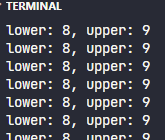
\includegraphics[scale=0.5]{images/binary-search-2}
	\caption{blah} % #TODO: think something to put here
	\label{fig:terminal-output-1}
	\end{subfigure}
	\begin{subfigure}{0.7\textwidth}
	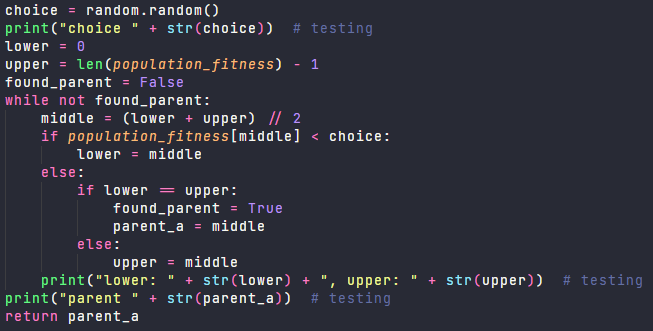
\includegraphics[scale=0.7]{images/binary-search-1}
	\caption{help} % #TODO: think of something to put here
	\label{fig:code-1}
	\end{subfigure}
\end{figure}  % #TODO: formatting

The relevant code is below in figure~\ref*{fig:code-2}

\begin{figure}[ht]
	\centering
	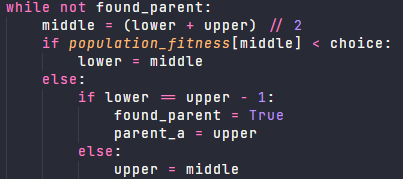
\includegraphics{images/binary-search-3}
	\caption{blah}  % #TODO: think of something to put here
	\label{fig:code-2}
\end{figure}

Changing the order of the \verb|if| \verb|else| statements solved the problem.

\begin{figure}[ht]
	\centering
	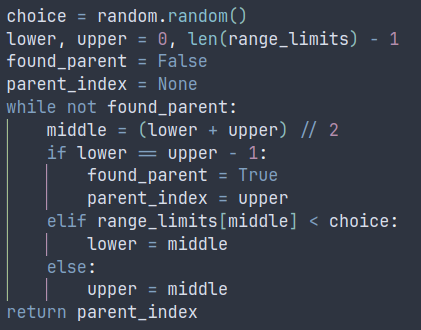
\includegraphics[scale=0.5]{images/binary-search-5}
	\caption{blah}  % #TODO: think of something to put here
	\label{fig:code-3}
\end{figure}

\newpage

% #TODO: changes made to algorithm
Another issue I encountered was that after thousands of generations, no valid 
solution was being found, and after further investigation, I discovered that the
population was converging to the same solution.

The first thing I tried doing to fix this was to the increase the chance of a
mutation occurring, as this does help to reduce convergence. 
This was simply done by decreasing the value of \verb|mutation-chance| in 
\verb|settings.json|.
This was not sufficient, and I also found that in several cases, improvements to
the fitness of the overall population (by means of fitter offspring) were 
diminished when they were mutated, as a mutation would often worsen the fitness 
of an individual.
I fixed this by calculating the fitness of the offspring immediately after the 
crossover phase.
If a member of the offspring has fitness that is the same as or worse than the
fitness of the worse parent, then it is mutated, otherwise it is not.
Some pseudocode for this is:

\begin{Verbatim}[numbers=left, fontsize=\footnotesize]
CheckFitness of offspring(return: offspringFitness)
mutateList := empty list
notMutateList := empty list
for solution in offspringFitness
    indexOffspring := index(offspringFitness(solution))
    if solution <= worstParentFitness:
        append offspring[indexOffspring] to mutateList
    else:
        append offspring[indexOffspring] to notMutateList
    end if
end for
\end{Verbatim}

For this, I also created another function that only returns the fitness values, 
and not a boolean for if there exists a valid solution, and that solution if it
does exist, because they are not needed.
The offspring that are not mutated are added to their own list so that they can
be recombined with the mutated offspring later.
Also note that \verb|SelectParents| also now returns \verb|worstParentFitness| 
so it can be used.

However, this did still not fix the problem of convergence. 
I then decided to change the number of parents involved in the crossover phase,
as it would help to diversify the ``gene pool''.
Additionally, only using two parents to generate very large populations (over 
100 individuals) would counteractive the benefit of the greater population size.
Therefore, it makes more sense for the number of parents to scale with the size
of the population.

So instead of selecting two parents using the previous ``spinner wheel'' method,
the half of the population with the better fitness will be chosen, and four 
offspring will be produced from a pair of parents.

Firstly, I decided to change how the fitness is calculated.
Because I do not need better fitness to be a larger number (as probability is no
longer being used choose the parents), the number of constraint violations is
not inverted, and instead that number is used to denote the fitness, meaning
that now, lower fitness is better, instead of before where higher fitness was 
better.
The pseudocode for this is now:

\begin{Verbatim}[numbers=left, fontsize=\footnotesize, tabsize=4]
function CheckFitness
input: population, teacherTimes
	
populationFitness := empty list
validSolutionBool := False
validSolution := None
for each solution in population:
	sort solution by timeSlot
	violations := 0
	for i in range(size(solution) - 1):
		if solution[i][0] == solution[i + 1][0]:
			if solution[i][1] == solution[i + 1][1]:
				violations := violations + 1
			end if
			if solution[i][2] == solution[i + 1][2]:
				violations := violations + 1
			end if
			if solution[i][4] == solution[i + 1][4]:
				violations := violations + 1
			end if
		end if
	end for
	for in range(size(solution)):
		timeSlot = solution[i][0]
		teacherNumber = solution[i][4]
		CONTINUE WHEN FINISHED CODE  #TODO: add code
	end for
	append violations to populationFitness
	if violations == 0:
		valid solution bool := True
		valid solution := solution
		break for loop
	end if
end for
return populationFitness, validSolution, validSolutionBool
\end{Verbatim}

The selection process for the parents is now greatly simplified, as they just
need to be sorted by their fitness, and then the best ones are selected.
However, it is not as simple as selecting half of population, if the size of the
population is an odd number, or if half of the population is an odd number (as 
there be one parent without a partner).
Therefore the size of the population needs to be a multiple of 4.
The pseudocode is now:

\begin{Verbatim}[numbers=left, fontsize=\footnotesize, tabsize=4]
function SelectParents
input: populationFitness, populationSize

parents := empty list
sortedFitness := populationFitness
sort sortedFitness  // sorts from low to high
for i in range(2 * ceiling(population_size / 4)):
    parent = sorted_fitness[0]
    append parent to parents
    if i == (2 * ceiling(population_size/4)) - 1:
        worst_parent_fitness = sorted_fitness[0]
	end if
    delete sorted_fitness[0]
end for
return parents, worst_parent_fitness
\end{Verbatim}

% change fitness calc and how parents were selected and change crossover

% using the same parent if they have the same fitness

% restructure how fitness is stored

% parent solutions were changing, narrow it down to when mutation was occurring

% deep copy to fix it

% #TODO: fufilled requirements

\chapter{Testing}  % #TODO: testing

\chapter{Evaluation}  % #TODO: evaluation 

\chapter{Conclusion}  % #TODO: conclusion

\renewcommand\bibname{References}
\bibliography{references.bib}

\appendix

\chapter{Tables and Figures} % #TODO: tables and figures appendix

\chapter{Pseudocode and Code Listings} % #TODO: pseudocode and code listings

\listoffigures

\chapter{Source Code}

\section{main.py}
\inputminted[linenos, fontsize=\footnotesize]{Python}{../main.py}

\section{ga.py}
\inputminted[linenos, fontsize=\footnotesize]{Python}{../modules/ga.py}

\section{initial{\textunderscore}population.py}
\inputminted[linenos, fontsize=\footnotesize]{Python}{
	../modules/initial_population.py}

\section{fitness{\textunderscore}function.py}
\inputminted[linenos, fontsize=\footnotesize]{Python}{
	../modules/fitness_function.py}

\section{selection.py}
\inputminted[linenos, fontsize=\footnotesize]{Python}{../modules/selection.py}

\section{crossover.py}
\inputminted[linenos, fontsize=\footnotesize]{Python}{../modules/crossover.py}

\section{mutation.py}
\inputminted[linenos, fontsize=\footnotesize]{Python}{../modules/mutation.py}

\end{document}
